\documentclass{article}
\usepackage{amsmath, amssymb}
\usepackage{array}
\usepackage{xcolor}
\usepackage{tikz}
\usetikzlibrary{arrows.meta}

\begin{document}

\section{Introduction}

Lecture 10 is about information complexity, but we will start with communication complexity.

\section{Communication Complexity}

We start with a function
\[
f: X \times Y \to Z
\]

\subsection{Examples}

We have $X,Y=\left\{0,1\right\}^n$, $Z=\left\{0,1\right\}$, and 
\[
f: \left\{0,1\right\}^n\times \left\{0,1\right\}^n \to \left\{0,1\right\}
\]
Player 1 gets $x\in X$ and player 2 gets $y\in Y$. They have to compute $f(x,y)$

Initially, the plays don't know each other's input. They run a communication complexity protocol. At the end, they both have to know the answer $f(x,y)$.

Each play has unlimited computational power. The issue is communication: How many communication bits the plays have to exchange between them in order to determine the answer.

Three examples of problems:
\begin{enumerate}
    \item \textbf{Equality:} Is $x=y$?
    \item \textbf{Set Disjointness:} Is there a coordinate $i$, such that, $x_i=y_i=1$?
    \item \textbf{Inner Product:} Compute $\sum_i x_i\cdot y_i \pmod 2$
\end{enumerate}
Sometimes we consider other computational tasks, with possibly more than one correct answer, rather than computation a function (e.g., search problems, promise problems).

\subsection{Deterministic Communication Complexity}

Deterministic communication protocols: In each step, one of the players sends one bit to the other player. This bit may depend on the previous communication and on the input of the player who sends it. At the end, they both have to know a value $\pi \left(x,y\right)$ (the output of the protocol). We require,
\[
\forall x\in X, y\in Y,\quad \pi(x,y)=f(x,y)
\]
The communication complexity of a protocol, $\operatorname{CC}(\pi)$, is the maximum (over all inputs) of the number of bits transmitted. The deterministic communication complexity of $f$, $\operatorname{CC}(f)$, is the minimum communication complexity of a protocol computes $f$.

\subsection{Probabilistic Communication Complexity}

The players can use random bits. The protocol is probabilistic. Each bit sent may depend on the random bits. The output $\pi(x,y)$ is now a random variable. We require,
\[
\forall x\in X, y\in Y, \quad \operatorname{P}(\pi(x,y)=f(x,y)) \geq 1-\epsilon
\]
$\epsilon$ is the probability of error (typically, some small constant).

The communication complexity of a protocol, $\operatorname{CC}(\pi)$, is the \textbf{maximum} (over all inputs and random strings) of the number of bits transmitted. The probabilistic communication complexity of $f$, $\operatorname{CC}(f)$, is the \textbf{minimum} communication complexity of a probabilistic protocol that computes $f$ with probability of error $\epsilon$.

Reducing $\epsilon\to \epsilon'$ is easy by repeating the protocol and taking majority.

\subsection{Public vs Private Randomness}

Public random bits can be viewed by both players. Private random bits can be viewed by only one of the players. In general, we can replace all private randomness with public randomness and the protocol still has the same success probability (trivial).

The other direction is also true: we can replace all public randomness with private randomness, if we allow additional $\mathcal{O}\left(\log n\right)$ bits of communication and a small increase in the probability of error (not hard but we will not prove).

We allow both public and private randomness as this will be needed when we talk about information complexity.

\subsection{Distributive Communication Complexity}

There is an underlying joint distribution $P_{X,Y}$ of the inputs $X,Y$ for the two players. The inputs are random variables, not necessarily independent. The protocol is deterministic. We require 
\[
P_{X,Y} \big(\pi\left(X,Y\right) = f(X,Y)\big)\geq 1-\epsilon
\]
We can also allow probabilistic protocols but this equivalent to the deterministic case because we can always take the random string with maximal success probability. When fixing the random string, we get a deterministic protocol. (A probabilistic protocol is just a convex combination (distribution over) probabilistic protocols).

When discussing distributive communication complexity, we sometimes consider the zero error case. (Similar to deterministic communication complexity when $X,Y$ are ...)

\subsection{Input Matrix}

It is sometimes helpful to view the function $f$ as a matrix:
\[
A_{x,y} = f(x,y)
\]
\textbf{Example:} Equality: $A$ is the identity matrix.

\subsection{Results}
\begin{itemize}
    \item CC(Equality) $= n+1$
    \item $\qquad$ Upper bound of $n+1$ true for every function to $\left\{0,1\right\}$
    \item $\operatorname{CC}_\epsilon\left(\text{Equality}\right)=\mathcal{O}(1)$ (public randomness)
    \item $\qquad$ Protocol: Players compare $\sum_{i} x_i\cdot z_i \pmod 2$ and $\sum_{i} y_i\cdot z_i \pmod 2$, for random $z_1\ldots, z_n$. (Can use error correcting codes to reduce randomness)
    \item $\operatorname{CC}_\epsilon\left(\text{Equality}\right)=\mathcal{O}(\log n)$ (private randomness)
    \item $\qquad$ Protocol: Players compare $x$ mod $p$ and $y$ mod $p$, for a random prime $p\in\left\{1,\ldots,n^2\right\}$. (Can use error correcting codes).
    \item $\operatorname{CC}_\epsilon\left(\text{Inner-Product}\right)=\Omega(n)$
    \item $\operatorname{CC}_\epsilon\left(\text{Set-Disjointness}\right)=\Omega(n)$
\end{itemize}

\subsection{Protocol as a Tree}

For simplicity, we sometimes assume that the players send bits alternately
% Preamble: \usepackage{tikz} \usetikzlibrary{arrows.meta}
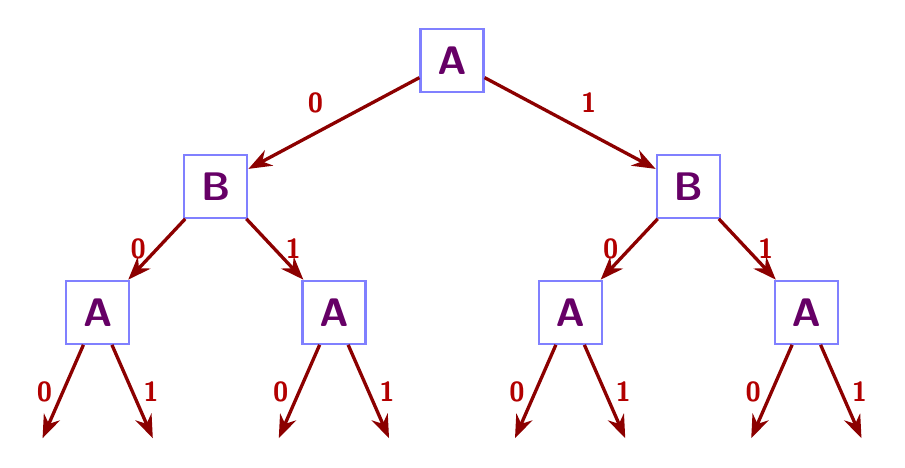
\begin{tikzpicture}[
  level distance=1.6cm,
  level 1/.style={sibling distance=6cm},
  level 2/.style={sibling distance=3cm},
  level 3/.style={sibling distance=1.4cm},
  state/.style={draw=blue!50, thick, text=violet!80!black,
                font=\sffamily\bfseries\Large, minimum size=0.8cm},
  edge from parent/.style={draw=red!55!black, very thick, -{Stealth}},
  lbl/.style={font=\sffamily\bfseries, text=red!70!black}
]
\node[state] {A}
  child { node[state] {B}
    child { node[state] {A}
      child { coordinate edge from parent node[lbl,left]  {0} }
      child { coordinate edge from parent node[lbl,right] {1} }
      edge from parent node[lbl,left] {0} }
    child { node[state] {A}
      child { coordinate edge from parent node[lbl,left]  {0} }
      child { coordinate edge from parent node[lbl,right] {1} }
      edge from parent node[lbl,right] {1} }
    edge from parent node[lbl,above left] {0} }
  child { node[state] {B}
    child { node[state] {A}
      child { coordinate edge from parent node[lbl,left]  {0} }
      child { coordinate edge from parent node[lbl,right] {1} }
      edge from parent node[lbl,left] {0} }
    child { node[state] {A}
      child { coordinate edge from parent node[lbl,left]  {0} }
      child { coordinate edge from parent node[lbl,right] {1} }
      edge from parent node[lbl,right] {1} }
    edge from parent node[lbl,above right] {1} };
\end{tikzpicture}

Bits sent by Alice may depend on $X$. Bits sent by Bob may depend on $Y$.

\subsection{Protocol as a Partitioning to Monochromatic Rectangles}

For simplicity, we sometimes assume that the players send bits alternately.
% Preamble: \usepackage{tikz}
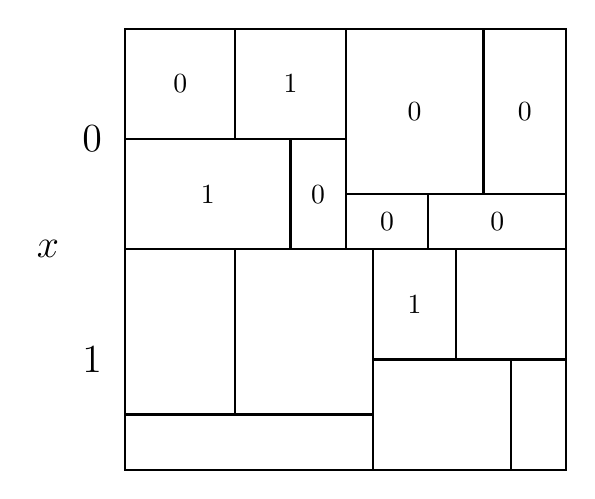
\begin{tikzpicture}[scale=0.7, thick]
  % Outer matrix (rows indexed by x, columns by y)
  \draw (0,0) rectangle (8,8);

  % --- Round 1: Alice splits rows (x = 0 on top, x = 1 on bottom)
  \draw (0,4) -- (8,4);

  % ===== Top half (x = 0) =====
  % Round 2: Bob splits columns
  \draw (4,4) -- (4,8);
  % Top-left quadrant
  \draw (0,6) -- (4,6);
  \draw (2,6) -- (2,8);
  \draw (3,4) -- (3,6);
  % Top-right quadrant
  \draw (4,5) -- (8,5);
  \draw (6.5,5) -- (6.5,8);
  \draw (5.5,4) -- (5.5,5);

  % Labels in the top half
  \node at (1,7)       {$0$};
  \node at (3,7)       {$1$};
  \node at (1.5,5)     {$1$};
  \node at (3.5,5)     {$0$};
  \node at (5.25,6.5)  {$0$};
  \node at (7.25,6.5)  {$0$};
  \node at (4.75,4.5)  {$0$};
  \node at (6.75,4.5)  {$0$};

  % ===== Bottom half (x = 1) =====
  \draw (4.5,0) -- (4.5,4);
  % Bottom-left
  \draw (0,1) -- (4.5,1);
  \draw (2,1) -- (2,4);
  % Bottom-right
  \draw (4.5,2) -- (8,2);
  \draw (6,2) -- (6,4);
  \draw (7,0) -- (7,2);

  % Labels in the bottom half (fill in the rest as needed)
  \node at (5.25,3) {$1$};

  % Row labels
  \node at (-0.6,6) {\Large $0$};
  \node at (-0.6,2) {\Large $1$};
  \node at (-1.4,4) {\Large $x$};
\end{tikzpicture}


\section{Information Complexity}

\subsection{The setup}

\begin{itemize}
    \item $X,Y$ are random inputs to Alice and Bob, with joint distribution $\mu = P_{X,Y}$.
    \item $R$: public random string; $R_A, R_B$: Alice's and Bob's private random strings
    \item $\pi$: probabilistic protocol between Alice and Bob 
    \item $M=\left(X,Y,R,R_A,R_B\right)$: transcript of the protocol: all bits transmitted
\end{itemize}
Let's assume for simplicity that the players send bits in an alternating fashion.

\textbf{Information Complexity measure the amount of information that the transcript gives about the inputs.}

There are two different types:
\begin{itemize}
    \item External Information Complexity
    \item Internal Information Complexity
\end{itemize}

\subsection{External Information Complexity}

Intuitively, external information complexity is the information that an external observer learns about the inputs $X,Y$ from the transcript $M$. The formal definition is 

\begin{align*}
    \text{Ext} &= \operatorname{I}\big(\left(X,Y\right); \left(M,R\right)\big)\\
    &= \operatorname{I}\big(\left(X,Y\right); R\big) + \operatorname{I}\big(\left(X,Y\right); M\mid R\big)\\
    &= 0 + \operatorname{I}\big(\left(X,Y\right); M\mid R\big)\\
    &= \operatorname{I}\big(\left(X,Y\right); M\mid R\big)
\end{align*}
because $R$ is independent from $X,Y$.

\subsection{Internal Information Complexity}

Intuitively, the information that the players learn about each other's input ($X$ or $Y$) from the transcript $M$.

Information that Alice learns about $Y$ from $M$ (conditioned on $X$):
\begin{align*}
    \operatorname{I}\big(Y; \left(M,R,R_A\right)\mid X\big) &= \operatorname{I}\big(Y; \left(M,R_A\right)\mid X, R)\\
    &= \operatorname{I}\big(Y; M\mid X,R\big) + \operatorname{I}\big(Y; R_A\mid M,X,R\big)\\
    &= \operatorname{I}\big(Y; M\mid X,R\big) + 0
\end{align*}
The first equality is as before. To show that $\operatorname{I}\big(Y; R_A\mid M,X,R\big)=0$, we use induction over the transcript: conditioned on $M,X,R$, we have that $Y,R_A$ are independent.

We define internal information complexity as 
\begin{align*}
    \text{Int} &= \operatorname{I}(Y; M\mid X, R) + \operatorname{I}(X; M\mid Y, R)
\end{align*}
Intuitively, the sum of the information that Alice learns about Bob and Bob learns about Alice.

\subsection{Information Complexity}

Now we have two definitions.
\begin{gather*}
    \text{Ext} = \operatorname{I}\big(\left(X,Y\right); M\mid R\big)\\
    \text{Int} = \operatorname{I}(Y; M\mid X, R) + \operatorname{I}(X; M\mid Y, R)
\end{gather*}

\subsubsection{Relations}
Always,
\[
\operatorname{CC}(\pi) \geq \text{Ext} \geq \text{Int}
\]
The first inequality is trivial. The second inequality is proved by induction over the transcript.

If $X,Y$ are independent, then 
\[
\text{Ext} = \text{Int}
\]

\subsection{Examples}

\begin{itemize}
    \item Alice and Bob send random bits...
    \item Alice and Bob send constant bits... 
    \item If $X_1=0$, Alice sends 0. If $X_1=1$, Alice sends 0 with probability $1-\epsilon$ and 1 with probability $\epsilon$. Both Ext and Int are very small.
\end{itemize}


\section{Zero-Error Information Complexity of AND}

\subsection{Setup}

Let's take $X,Y\in\left\{0,1\right\}$: independent and uniformly distributed. Alice and Bob need to compute $X\wedge Y$ with no error. What is the minimal Ext and Int?

Since $X,Y$ are independent, Ext=Int.

\subsubsection{Observation}

If Alice and Bob both learn\footnote{So if Alice has $0$ and learns the output is $0$, she doesn't know what Bob has.} $X\wedge Y$, they each learn the input of the other with probability $\frac{1}{2}$. Together, they learn $\frac{1}{2}+\frac{1}{2}=1$ bit, just by learning the output. Thus, $\operatorname{Int}\geq 1$. Hence $\operatorname{Ext}\geq 1$.

\subsubsection{Observation}

$\operatorname{CC}\left(\text{And}\right)=2$. Hence, Ext=Int$\leq 2$.

Is there a protocol with $\operatorname{Ext},\operatorname{Int}\leq 2$?

\subsubsection{Protocol}

Alice sends $X$. Bob sends back $X\wedge Y$. 
\[
\operatorname{Ext}=\operatorname{Int}=1.5
\]
Thus, $1\leq \operatorname{Ext,Int}\leq 1.5$

\subsection{4 Messages Protocol (ABAB)}

The point is that the communication complexity is higher than before, but the information complexity is lower! What the hell?!?

$X,Y\in_R \left\{0,1\right\}$. Compute $X\wedge Y$. We have Ext=Int. What is the minimal Ext, Int?

\begin{itemize}
    \item If $X=0$, Alice chooses $i\in_R \left\{1,3\right\}$ (the round in which she reveals $X=0$, and then the game ends)
    \item If $Y=0$, Bob chooses $j\in_R \left\{2,4\right\}$ (the round in which he reveals $Y=0$, and then the game ends)
\end{itemize}

\begin{center}
\renewcommand{\arraystretch}{1.3}
\begin{tabular}{l l c l l}
\textbf{First Round:}  & $X=1$            & $\to$ & $A$ sends $1$ & \\
                       & $X=0,\ i=3$      & $\to$ & $A$ sends $1$ & \\
                       & $X=0,\ i=1$      & $\to$ & $A$ sends $0$ & Stop \\
\textbf{Second Round:} & $Y=1$            & $\to$ & $B$ sends $1$ & \\
                       & $Y=0,\ j=4$      & $\to$ & $B$ sends $1$ & \\
                       & $Y=0,\ j=2$      & $\to$ & $B$ sends $0$ & Stop \\
\textbf{Third Round:}  & $X=1$            & $\to$ & $A$ sends $1$ & \\
                       & $X=0$            & $\to$ & $A$ sends $0$ & Stop \\
\textbf{Fourth Round:} & $Y=1$            & $\to$ & $B$ sends $1$ & Stop \\
                       & $Y=0$            & $\to$ & $B$ sends $0$ & Stop
\end{tabular}
\end{center}

\begin{center}
\renewcommand{\arraystretch}{1.4}
\begin{tabular}{l c l}
\textbf{Probability} & \textbf{Transcript} & \textbf{External Observer learned} \\
\hline
$\frac{1}{4}$                                        & $0$    & $1$ \\
$\frac{3}{4}\cdot\frac{1}{4}$                        & $10$   & $1 + \left(1 - \operatorname{H}\!\left(\frac{1}{3},\frac{2}{3}\right)\right)$ \\
$\frac{3}{4}\cdot\frac{3}{4}\cdot\frac{1}{3}$        & $110$  & $1 + \left(1 - \operatorname{H}\!\left(\frac{1}{3},\frac{2}{3}\right)\right)$ \\
$\frac{1}{8}$                                        & $1110$ & $2$ \\
$\frac{1}{4}$                                        & $1111$ & $2$
\end{tabular}
\end{center}

\[
\text{Ext} = \text{Int} = 1 + \frac{3}{8}\cdot 1 + \frac{3}{8}\cdot \left(1- \operatorname{H}\left(\frac{1}{3}, \frac{2}{3}\right)\right) < 1.5
\]

\subsection{Best Protocol}

$X,Y\in_R \left\{0,1\right\}$. Compute $X\wedge Y$. $\text{Ext}=\text{Int}$. What is the minimal Ext, Int? We take $n\to \infty$. $n$ is even and ABAB... 

\begin{itemize}
    \item If $X=0$, Alice chooses a random odd $i\in\left\{1,\ldots,n\right\}$ (the round in which she reveals $X=0$, and then the game ends).
    \item If $Y=0$, Bob chooses a random even $j\in \left\{1,\ldots,n\right\}$ (the round in which he reveals $Y=0$, and then the game ends).
    \item If $X=1$, Alice sends $1$ in all rounds. If $X=0$, Alice sends 1 until round $i$ and $0$ in round $i$ and then the protocol stops.
    \item If $Y=1$, Bob sends 1 in all rounds. If $Y=0$, Bob sends 1 until round $j$ and then the protocol stops
\end{itemize}
The probability for $X=1$ and $Y=1$ slowly increases if the protocol didn't stop. The information is slowly released.

We can think about this as two people trying to figure out if they like each other without hurting the other's feelings.

\subsection{Continuous Protocol (Equivalent)}

$X,Y\in_R \left\{0,1\right\}$. Compute $X\wedge Y$. Ext=Int. What is the minimal Ext, Int?

\begin{itemize}
    \item If $X=0$, Alice chooses a random $t_A\in[0,1]$ (the time at which she reveals $X=0$, and then the game ends).
    \item If $Y=0$, Bob chooses a random $t_B\in[0,1]$ (the time at which he reveals $Y=0$, and then the game ends).
    \item A clock starts to run (continuously) from time $0$ to $1$.
    \item If $X=0$, Alice raises her hand at time $t_A$. The protocol stops. Answer: $0$.
    \item If $Y=0$, Bob raises his hand at time $t_B$. The protocol stops. Answer: $0$.
    \item If no one has raised a hand by time $1$, the protocol stops. Answer: $1$.
    \item The probability that $X=1$ and $Y=1$ slowly increases if the protocol hasn't stopped. The information is released slowly.
\end{itemize}

\subsection{Reasons to Study Information Complexity}

\begin{enumerate}
    \item Lower bounds for communication complexity and other models
    \item Relations to streaming complexity and other models
    \item Information theoretic privacy 
    \item Direct sum problems: Int is additive for two communication tasks
    \item Compression problem: If Int, Ext are small, is there a (possibly different) protocol with small CC?
\end{enumerate}



\end{document}